\documentclass[a4paper, 11pt]{article}
\usepackage{comment} % enables the use of multi-line comments (\ifx \fi) 
\usepackage{lipsum} %This package just generates Lorem Ipsum filler text. 
\usepackage{fullpage} % changes the margin
\usepackage{amsmath}
\usepackage{kbordermatrix}
\usepackage{hanging}
\usepackage{graphicx}
\graphicspath{ {images/} }
\begin{document}
%Header-Make sure you update this information!!!!
\noindent
\large\textbf{Midterm}.\\
\normalsize CAPP 30254 \hfill Camilo Arias \\
Prof. Rayid Ghani\hfill Date: 05/13/2019 \\\\

\section*{Short answers}

\begin{enumerate}
\item You’re asked to predict the probability that the unemployment rate will go down next quarter for each of the neighborhoods in Chicago. Which model would you prefer to use?

\textbf{Logistic Regression}

I would prefer to use Logistic Regression. It actually provides a probability of success, whereas SVM provides the distance to the division hyperplane.

\item Do you have to do anything special with the data or features for this problem with the model you chose in 1?

I would need to create a dummy variable with value of one if unemployment rate decreased next quarter for every block. 

\item What is the training error (error on the training set) for a 1-NN classifier?

The error rate is zero because each observation in the train set will be predicted with its own label.

\item What is the Leave-one-out cross validation error for k nearest neighbor on the following data set? List any assumptions you may be making.

For $K = 1$, the average error among the 5 cross validations is 0\\
For $K = 3$ the average error among the 5 cross validations is 0.8.\\
I am assuming that the farthest $-$ for the two $+$ in the middle is closest than the $+$ on the bottom. All but the bottom observation would be predicted incorrectly

\item Which of the following classifiers are appropriate to use for the following data set? Why?

\textbf{Decision Tree}

Decision Tree would be able to capture the non linear relation between the classification and the x and y values by splitting first in one variable and then in the other. SVM and Logistic Regression would try to fit a linear function.

\item You are being asked to build a model to predict which children in Chicago are at risk of Asthma attacks. You create 1000 features (all continuous) but you find out after exploring the data and talking to public health and medical experts that ~10 of them are useful and relevant for the prediction problem. Which of the classifiers below would you choose? And why?

\textbf{Decision Trees}

The decision Tree will be able to identify the most important variables, in terms of increasing purity split after split. KNN considers all variables equally, without evaluating if they actually contribute to the classification problem. 


\item Does Boosting give you a linear classifier? Why or why not?

It would normally not give a linear classifier. Boosting iteratively increases the weights of the misclassified observations and fits a new model. The final aggregated model is a combination of each of the models, which will solve for the nonlinearities in the data if the decision model is a linear classifier. Only if data was perfectly classified in the initial model with a linear model, the result of boosting will be linear.

\item Can boosting perfectly classify all the training examples for any given data set? Why or why not?

No it generally cannot, because when you train a new model by increasing weights of the misclassified, the ones that were correctly classified will get less importance and the model will probably miss them. The only case would be if data were linearly separable. 

\item If you have a data set with 10 variables, each of them binary, with a binary target variable (label). You are asked to build a decision tree. If you didn’t use a greedy approach and built all possible trees on this data set (without pruning or limiting the depth), how many trees would you build?

Any tree will have a height of 10, with $2^10$ split labels. With 10 features, there will be $2^{2^{10}}$ possible trees, equivalent to $2^{1024}$.

\item You are reading a paper for a new method to identify people at risk of pre-term and adverse births.. The reported accuracy is 89.4\% and the precision at the top 10\% is 56\%. Are those numbers high enough to justify you replicating the method in your project (please explain your answer in 1-2 sentences)?

\textbf{Maybe}\\
The accuracy is no surprising because a naive classifier would have 88\% accuracy since only 12\% of the births are premature in US. However, precision is much better than the one resulting from selecting 10\% at random. We would need more information about the baseline.

\item A Random Forest will always perform better than a decision tree on the same data set.

\textbf{False}\\
A random forest will not be better than a Decision Tree in some cases. One case is if very few variables are relevant. A single decision tree will always pick them while a random forest with a small $m$ will miss them many itmes.
\\

\textit{You need to build a model to predict re-entry into a social service program. A colleague suggests building a separate model for males and females while another colleague insists you just need to build one combined model.}
\item When will separate models be more appropriate?

A separate model will make more sense in some cases. If with the model I would then intervene in the cases with the highest probability, and either males or females have systematically higher rates of re-entry, then the recall at x\% will be very bad for the gender with low rates if we estimate a combined model. The will come form the nature of the application. If decisions will be made separately, it would make sense to estimate different models. If the cost or benefits of the a correct precision differ by gender, this would also be a good argument.

Moreover, if we have different features for males and females or if the relation is different between the features and re-entry a separate estimation could make sense. For example, if the males presented a more linear relation while the females presented non linearities, then it could make sense to train a liner classifier for males and decision tree for females. 

\item When will a combined model be more appropriate?

Generally, if the use of the model will be the same and the data is the same, it will be better to estimate a combined model. Otherwise, why not estimate different models by height? If we don't care about recall in both genders, a combined model will output the people with the highest risk and will have the greatest prediction. This would make sense if the cost of false positives were too high, or if decisions were to be made in the same place.
\item What are the pros and cons of each approach?

The pros of estimating the same model are higher precision, easier maintenance, easier to test and to train because only one pipeline, and in general, better training. 

The pros of estimating different models are ensuring some level of recall for each gender. If predictions will be made separately, different models would work. Also, testing different specifications for each gender would be possible

\item What would you do?

I would estimate the the three models and I would compare the results. I would see the tradeoff between precision and recall. If results are too unbalanced in terms of recall for one gender, then maybe different models would work. If the goal is predicting the ones at the highest risk, then maybe I would keep the combined.
\end{enumerate}

\section*{Section B}

\begin{enumerate}
\item Decision Trees
	\begin{enumerate}
		\item What will be the random baseline accuracy for this data set?
		
		The expected random baseline will be $\frac{6 * 6/10 + 4 * 4 / 10}{10} = 52/100 = 0.52$
		\item Calculate the entropy for the target variable, EnergyConsumption
		
		\begin{gather*}
		entropy = -p \log(p) - (1-p)\log(1-p) = \\
		-6/10 \log(6/10) - (4/10)\log(4/10) = 0.67
		\end{gather*}
		
		\item Now calculate the Information Gain if you do a split on the feature “Home Insulation“
		
		$$IG = entropy(parent) - [p(c_{1}) entropy(c_{1}) + p(c_{2}) entropy(c_{2}) + ...]$$
		\begin{gather*}
		entropy(Poor) = -4/5\log(4/5) - 1/5\log(1/5) = 0.5\\
		entropy(Excellent) = 3/5 \log(3/5) - (2/5)\log(2/5) = 0.67\\
		p(poor) = p(Excellent) = 0.5
		\end{gather*}
		$$IG = 0.67 - [0.5(0.5 + 0.67)] = 0.086$$
		
		\item  Using the data above, construct a two-level decision tree that can be used to predict Energy Consumption. Don’t worry about overfitting or pruning. You can use a simple algorithm such as ID3 (using information gain as the splitting criterion).
		
		
		\textbf{Level 1:}
		\begin{gather*}
		IG_{HomeSize}= 0.007 \\
		IG_{HomeInsulation} = 0.086\\
		IG_{Temp} = 0.146
		\end{gather*}
		\textbf{The best split for the first node is Temperature}\\
		
		\textbf{Level 2:}
		\begin{itemize}
			\item Cool temperature node
			\begin{gather*}
				IG_{HomeInsulation} = 0.29 \\
				IG_{HomeSize} = 0.29
			\end{gather*}
			Best split for Cool temperature node is random.
			\item Mild temperature node
			\begin{gather*}
				IG_{HomeInsulation} = 0 \\
				IG_{HomeSize} = 0
			\end{gather*}
			Best split for Mild temperature node is no split.
			\item Hot temperature node
			\begin{gather*}
				IG_{HomeInsulation} = 0.17 \\
				IG_{HomeSize} = 0.63
			\end{gather*}
			Best split for Hot temperature node is Home Size
		\end{itemize}
		
		Final Tree:\\
		if temp == Cool:\\
		-----if HomeInsulation == Poor:\\
		----------EnergyConsumption = High \\
		-----else HomeInsulation == Excellent : \\
		----------EnergyConsumption = Low\\
		elif temp == Mild:\\
		-----EnergyConsumption = High\\
		else temp == Hot:\\
		-----if HomeSize == Small:\\
		----------EnergyConsumption = Low\\
		-----elif HomeSize == Medium:\\
		----------EnergyConsumption = Low\\
		-----else HomeSize == Large:\\
		----------EnergyConsumption = High\\
\end{enumerate}
\item Evaluation 1
	\begin{enumerate}
	\item What is the accuracy of the SVM on this set? 
	
	\textit{Threshold: 0.4}\\

	\begin{tabular}{ c | c | c | c | c }
	Id & Prob SVM & Prob LR & True & Pred SVM \\
	\hline
	1 & 0.98 & 0.85 & 1 & 1 \\
	2 & 0.2 & 0.3 & 0 & 0 \\
	3 & 0.1 & 0.22 & 0 & 0 \\ 
	4 & 0.99 & 0.9 & 1 & 1 \\
	5 & 0.55 & 0.4 & 0 & 1 \\
	6 & 0.05 & 0.2 & 0 & 0 \\
	7 & 0.4 & 0.1 & 1 & 0 \\
	8 & 0.35 & 0.35 & 0 & 0 \\
	9 & 0.65 & 0.81 & 0 & 1 \\
	10 & 0.75 & 0.5 & 1 & 1 \\
	\hline
	\end{tabular}\\

Accuracy at threshold of 0.4 is 0.7.\\

	\item Plot precision and recall curves for both classifiers
	\begin{figure}[hbt!]
    	\centering
     	\caption{Precision and Recall SVM and LR}
     	\label{fig:examples}
     	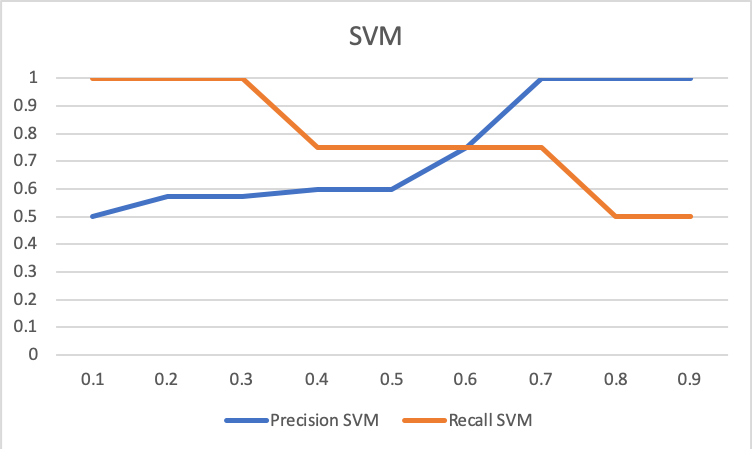
\includegraphics[scale = 0.7]{pre_rec_SVM}
	\\
     	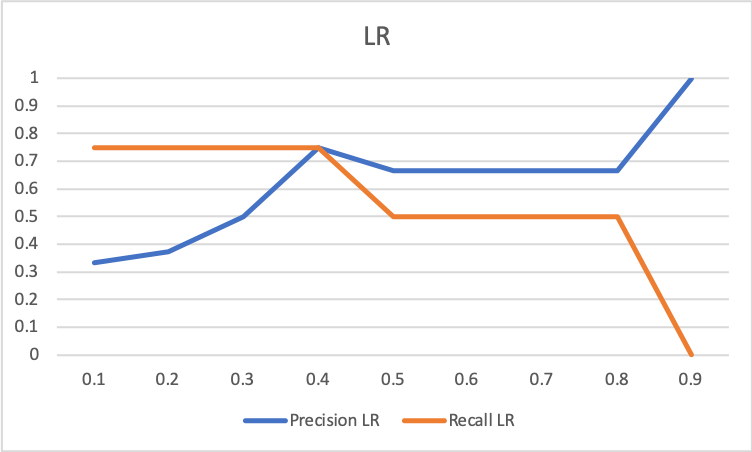
\includegraphics[scale = 0.7]{pre_rec_LR}
\end{figure}\\

	\item Which model is better
	
	Assuming we were predicting the events to intervene as a public agency, with budget constraints that limit the number of interventions, I would prefer SVM over LR. For all thresholds, precision is greater, and thus recall is also better. 
	\end{enumerate}
	
\item Evaluation 2
\begin{enumerate}
\item How would you explain what’s happening at the beginning of the graph to someone who’s not a machine learning expert?

In the beginning of the graph, we are classifying as TRUE under 5\% of the population. The graph shows the percentage of real TRUE of the observations I predicted as TRUE. Since in the beginning of the graph, the total I predicted to be TRUE is a very small number, it is very sensitive to one wrong prediction. 

\item What could be the reason for that behavior?
Possible, a couple of observations were assigned a high probability of being TRUE when they are not, which is creating that behavior. The importance of these observation diminishes as the number of predicted TRUE increases. There may be some non linearities that the model is not capturing. 

\item How would you solve it?

I would try a couple of things. The first one, if possible, would be to create more features or to increase the data. Probably this won't be possible. The second one would be to try different specifications of the model, as well as some non linear models. Finally, I would try boosting to overweight those observations that are not being correctly classified.

\end{enumerate}

\item Evaluation 3
\begin{enumerate}
\item What can you say about the behavior of Logistic Regression as you vary the parameters?

The table shows that Logistic Regression in this case has a better precision when fitted with penalty l2 than penalty l1. In terms of c, the Inverse regularization parameter, I don't see a clear pattern.

\item Which specific model would you select to deploy (and why)? going forward if you wanted to prioritize the 5\% highest risk?\\
I would select the LR with penalty l2 and C - 0.1 because that is the one with highest precision. When the threshold is fixed, precision is the key metric, since it also implies higher recall. 

\item Which specific model would you select to deploy (and why)? going forward if resources were yet to be determined.
I would stick with the same model. It has the highest Area Under the ROC curve, which reflects the overall performance of the model over the different thresholds. Also, the model has also the highest precision at 2-0\% and the second highest at 10\%.


\end{enumerate}

\item Communicating your results
\begin{enumerate}

\item

Dear Administrator,

Thanks for reaching out to me. I understand the doubts you have about this result. Let me explain what that number indicates. The purpose of our model is to identify the students at the highest risk of not graduating. The resulting score, in the case of Jenny of 50, is used to compare her risk with the risk of the other students. The number does not indicate that Jenny has a 50\% chance of dropping out before graduating. It might be the case that Jenny with a score of 50 is among the students with lowest probability of not graduating. However, it could also be the case that our model actually predicts Jenny to be at a high risk of dropping out. In this case, the characteristics of Jenny that you know make her a great student might not be among the characteristics we used in our model. In the same line, Jenny might share some characteristics with students that have dropped in previous years, and error like this will always be part of the prediction task.

\item
To confirm the accuracy of the model, please see the ranking of Jenny. If you know the school ability of the other students as you know it for Jenny, you might see a coherent ranking between the class. You can directly test our model with a Student you know is at a high risk of not graduating, and confirm that the score is higher than the score of Jenny. If it is the case that Jenny was predicted too high, please do the same exercise with other successful students. If you encounter big differences, please let me know.

Best,
Camilo

\end{enumerate}
\end{enumerate}
\section*{Section c: Solving a New Problem}
\begin{enumerate}

\item How would you formulate this as a machine learning problem? (is it supervised
learning or unsupervised learning? If it’s the former, what’s the label? What is each
row in your training date? How would you get the training data?

Let's think I have two dataframes. One of them my main data, and one external data I want to link. Both have name, last name, date of birth, gender, address. My first step will be to do some matchings by hand. I would do some research with the public agencies, and some very detailed analysis of the data to find a match for 10\% of my main data (assuming I had the resources to do that). 

This would be a supervised learning problem. The train and test set will be portions of the cross product of the 10\% I matched and the secondary dataframe. There will be one column indicating if a match was identified or not. My outcome variable will be that variable, which categorized the task as supervised learning.

I will then fit the model maximizing precision. I care that the links I claim to exist, really exist. Linking data from a different person can be very costly in my policy application of crime. Finally, I will deploy the model to the cross product of the other 90\% of the data and the secondary dataframe.

\item The features of my data will be the following:
\begin{itemize}
\item dummies for edit distance from name 1 to name 2.
\item dummies for edit distance from address1 and address 2.
\item dummies for equal or unequal gender1 and gender2.
\item dummies for equal date of birth
\item dummies for same day and same month but different year in dates of birth.
\item dummies for same year and same month but different day in dates of birth.
\item dummies for same day and same year but different month in dates of birth.
\item dummies for string comparison but with an alternative string distance metric. In case they are continuous, I would categorize them and then convert them to dummies.
\end{itemize}
\item What models would I use?
I would expect the model to be fairly linear. All variables seem to have homogeneous effect of the probability of a link. I would mainly try Logistic Regression, SVM. I would also see a Decision Tree to analyze its performance. I don't think Random Forest is justifies because we don't have many features. Bagging and Boosting could improve the precision is there are some non linearities present.

\item What evaluation metric?
I would mainly focus on precision. I want the links that I predict to be real links because linking information from a different person in this policy application is unethical. I think the distribution of scores will have two peaks, one close to zero and one close to one. That will be the key to select the threshold. 

\item Would you expect the machine learning solution to work better than exact
matching or “fuzzy”/approximate matching rules? Why or why not?
Exact matching will miss many links because different ways of recording names and dates. Exact link will be the case of selecting the threshold extremely high. Machine Learning would be better because some not exact links will be discovered. I also think ML would work better than approximate matching rules because the rules will be inferred from the training data, not from a prior of the researcher. Also, more complex rules will be created by Machine Learning. The approaches could work very similarly, with ML having a higher computational cost. But probably, ML will add to the precision of the classifier.
\end{enumerate}
\end{document}

